\section{Godiva rank sweep}
\label{sec:godiva}

Godiva (HEU-MET-FAST-001) is a bare $93.71\%$-enriched
uranium metal sphere. Its fast, leakage-dominated spectrum
places no demand on the RRR.
Table~\ref{tab:keff_godiva_desktop} reports the desktop ten-seed
sweep; laptop five-seed results are in
Table~\ref{tab:keff_godiva}.

\begin{table}[htb]
\centering
\caption{Godiva $k_\text{eff}$, laptop Ryzen~$7$. Five seeds,
$50$ batches, $10\,000$ particles per batch.}
\label{tab:keff_godiva}
\begin{tabular}{@{}lccccc@{}}
\toprule
Mode & rank & $k_\text{eff}$ & $\sigma_\text{seed}$ & ns/particle & time/seed (s) \\
\midrule
Pointwise table & ---  & $1.00523$ & $0.00235$ & $2\,385$ & $3.58$ \\
SVD & $2$  & $1.00448$ & $0.00165$ & $\mathbf{864}$  & $\mathbf{1.30}$ \\
SVD & $3$  & $1.00559$ & $0.00094$ & $1\,457$ & $2.19$ \\
SVD & $4$  & $1.00638$ & $0.00166$ & $1\,182$ & $1.77$ \\
SVD & $5$  & $1.00592$ & $0.00178$ & $1\,403$ & $2.10$ \\
SVD & $6$  & $1.00489$ & $0.00205$ & $1\,424$ & $2.14$ \\
\bottomrule
\end{tabular}
\end{table}

\begin{table}[htb]
\centering
\caption{Godiva, desktop Ryzen~$9800$X3D + RTX~$3080$. Ten
seeds, $150$ batches ($20$ inactive), $50\,000$ particles per
batch.}
\label{tab:keff_godiva_desktop}
\begin{tabular}{@{}lccccc@{}}
\toprule
Mode & rank & $k_\text{eff}$ & $\sigma_\text{seed}$ & ns/particle & time/seed (s) \\
\midrule
CPU table           & ---  & $1.00579$ & $0.00046$ & $1\,214$ & $7.89$ \\
CPU SVD             & $2$  & $1.00477$ & $0.00055$ & $1\,289$ & $8.38$ \\
CPU SVD             & $3$  & $1.00547$ & $0.00031$ & $1\,316$ & $8.56$ \\
CPU SVD             & $4$  & $1.00523$ & $0.00055$ & $1\,369$ & $8.89$ \\
CPU SVD             & $5$  & $1.00507$ & $0.00065$ & $1\,426$ & $9.27$ \\
CPU SVD             & $6$  & $1.00524$ & $0.00071$ & $1\,558$ & $10.13$ \\
GPU pointwise       & ---  & $1.00590$ & $0.00037$ & $278.5$  & $1.81$ \\
GPU SVD             & $5$  & $1.00536$ & $0.00046$ & $357.0$  & $2.32$ \\
\bottomrule
\end{tabular}
\end{table}

On laptop Godiva, SVD rank-$2$ is $2.8\times$ faster than the
pointwise table ($864$ vs $2\,385$~ns/p) at a modest
$75$~pcm bias. On desktop Godiva, the ranking inverts: the
V-cache L3 makes the table's per-particle cost ($1\,214$~ns)
lower than low-rank SVD ($1\,289$~ns at $k=2$). CPU SVD
ranks $3$--$6$ sit within $2$--$3\,\mathrm{SEM}$ of the
table; rank-$2$ is $102$~pcm low ($\sim\!4\,\mathrm{SEM}$).
GPU pointwise at $278.5$~ns/p is $4.4\times$ the desktop CPU
table and $8.6\times$ the laptop CPU table; GPU SVD rank-$5$
at $357$~ns/p is slightly slower, discussed in
Sec.~\ref{sec:gpu}.

Figure~\ref{fig:pareto_godiva} shows the laptop Pareto and
Figure~\ref{fig:throughput_godiva} shows the full desktop
rank sweep (throughput plus $k_\text{eff}$).

\begin{figure}[htb]
\centering
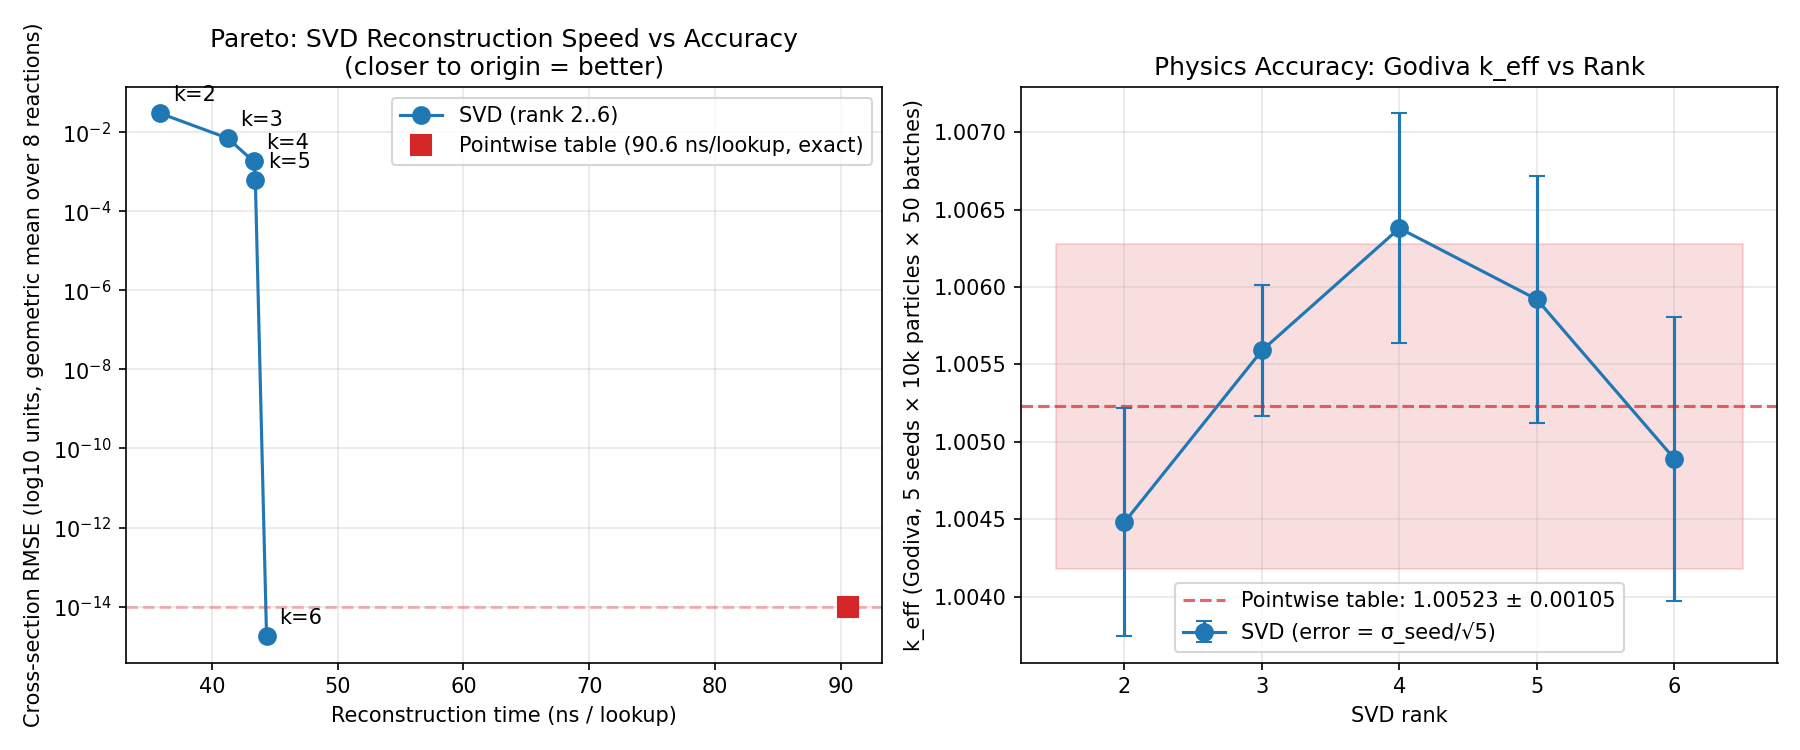
\includegraphics[width=0.99\textwidth]{../outputs/pareto/pareto.png}
\caption{Godiva, laptop. \emph{Left:} XS reconstruction cost
against RMSE (geometric mean over eight reactions).
\emph{Right:} $k_\text{eff}$ versus SVD rank, SEM error bars
over five seeds. Horizontal band: pointwise-table reference
in the same engine.}
\label{fig:pareto_godiva}
\end{figure}

\begin{figure}[htb]
\centering
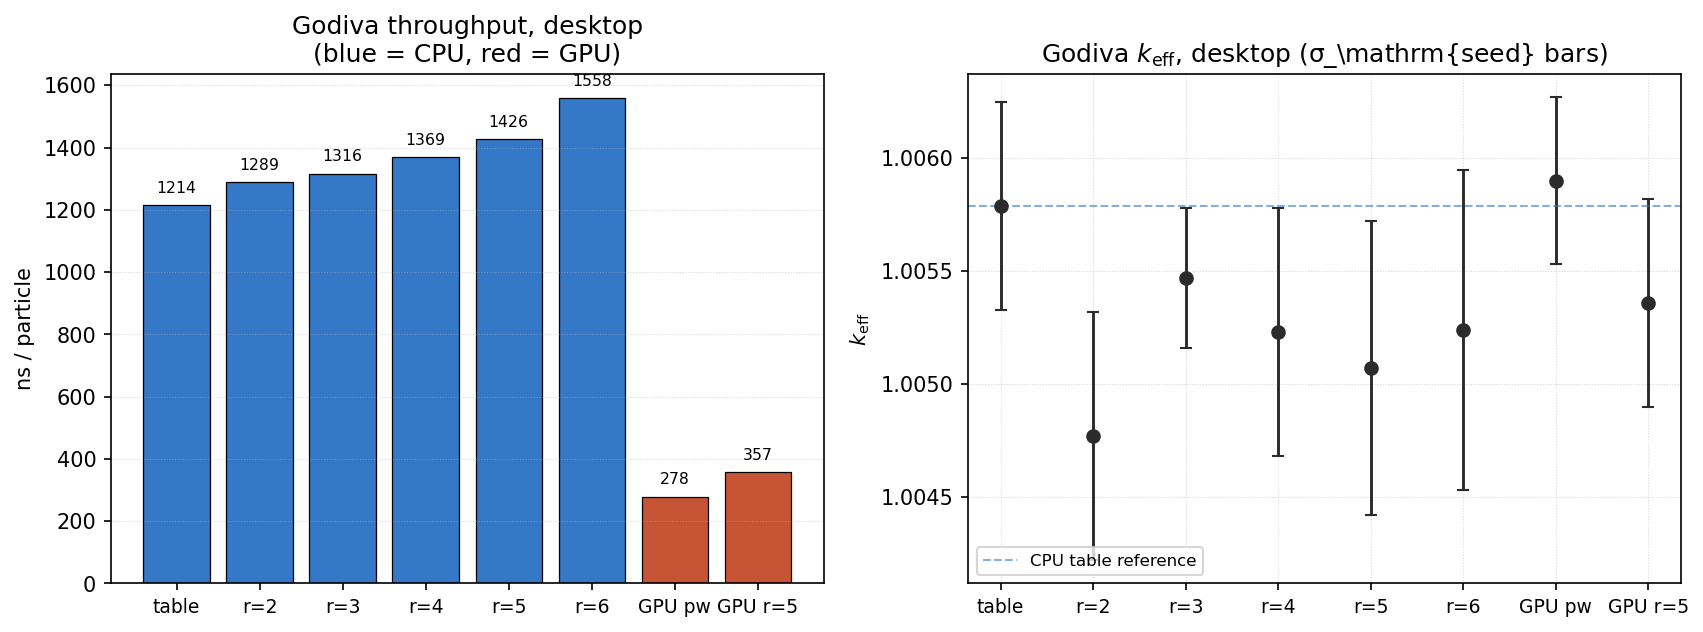
\includegraphics[width=0.99\textwidth]{../outputs/pareto/throughput_godiva.png}
\caption{Godiva, desktop rank sweep (ten seeds).
\emph{Left:} ns/particle per provider (blue CPU, red GPU).
\emph{Right:} $k_\text{eff}$ per provider, $\sigma_\text{seed}$
error bars; dashed line is the CPU-table baseline
$1.00579$.}
\label{fig:throughput_godiva}
\end{figure}

%% ============================================================
